
\documentclass[11pt,a4paper,onecolumn]{article}
\usepackage{qc}

%---------设定区结束----------
%---------预定设置区----------
\title{%
	\heiti \huge \vspace{-50pt} 量子化学原理与应用笔记 \\ \LaTeX 模板}
\author{John Doe}
%\institute{复旦大学}


\begin{document}
\bibliographystyle{JAmChemSoc}

\maketitle
\vspace{-10pt}

%\tableofcontents

%---------正  文  区----------

\section{公式}

~\\
有编号公式
\begin{equation}
  \hat A u = v
\end{equation}
无编号公式
\begin{equation*}
  c u, f u, \frac{\partial}{\partial x} u, \sqrt{u}
\end{equation*}
多行公式,分别编号
\begin{align}
\ev{A} &= \int \psi^* \hat A \psi \dd x \\
\ev{A}^* &= \qty(\int \psi^* \hat A \psi \dd x )^* = \int (\hat A \psi)^* \psi \dd x
\end{align}
多行公式,只编号一次
\begin{align}
\pdv{t} |\Psi(x,t)|^2  &= \pdv{\Psi^*}{t}\Psi + \Psi^*\pdv{\Psi}{t}  
= \Psi \qty(-\dfrac{i\hbar}{2m} \pdv[2]{x} \Psi + \dfrac{i}{\hbar} V(x) \Psi) + \Psi^* \qty(\dfrac{i\hbar}{2m} \pdv[2]{x} \Psi - \dfrac{i}{\hbar} V(x) \Psi) \notag\\
&= \dfrac{i\hbar}{2m} \qty[\Psi^*\pdv[2]{\Psi}{x} - \Psi\pdv[2]{\Psi^*}{x}] \notag\\
&= \dfrac{i\hbar}{2m} \pdv{x} \qty[\Psi^*\pdv{\Psi}{x} - \Psi\pdv{\Psi^*}{x}]
\end{align}
单行多行混合公式
\begin{equation}\label{eq.finite-square-potential}
V(x) = \left\{
\mqty{
& 0, && x \in (-\infty, 0) && \text{Block I} \\
& V_0, && x \in [0, l] && \text{Block II} \\
& 0, && x \in (l, +\infty) && \text{Block III}
}
\right.
\end{equation}
有编号列表
\begin{enumerate}[nosep]
	\item 和与差
	\item 乘法
	\item 等价算符
	\item 基本算符
	\item 逆
	\item 对易子
\end{enumerate}
无编号列表
	\begin{itemize}[nosep]
	\item 三维:$ s < \frac{3}{2} $
	\item  二维:$ s < 1 $
	\item  一维:$ s < \frac{1}{2} $
\end{itemize}


\subsection{数学和物理符号}

基本符号
%\begin{note}
\begin{lstlisting}[language=TeX]
$ \hbar, \oint, \prod, \forall,  \nabla,\cdots,  \therefore $\\
$ \hat A , \mathbb{R}, \Re, \ell$\\
$ \neq, \gg, \ll, \approx, \propto, \rightarrow, \Rightarrow, \leftrightarrow$\\
$ \sin, \arcsin, \sinh, \ln, \exp $
\end{lstlisting}
%\end{note}
$ \hbar, \oint, \prod, \forall,  \nabla,\cdots,  \therefore $\\
$ \hat A , \mathbb{R}, \Re, \ell$\\
$ \neq, \gg, \ll, \approx, \propto, \rightarrow, \Rightarrow, \leftrightarrow$\\
$ \sin, \arcsin, \sinh, \ln, \exp $
\\

physics包中的符号
\begin{lstlisting}[language=TeX]
\begin{equation}
\dv{x}, \dv{\psi}{x}, \dv[2]{\psi}{x}, \pdv{x}, \pdv[2]{x} , \int \dd x
\end{equation}
\begin{equation}
\bra{\varphi}, \ket{\phi}, \ev{\hat p}
\end{equation}  
\begin{equation}
\qty(  \dfrac{x}{y} ), \qty[ \dfrac{x}{y} ], \qty{\dfrac{x}{y} }, \qty| \dfrac{x}{y} |
\end{equation}
\begin{equation}
\mqty( a & b \\ c & d ), \mqty| a & b \\ c & d |
\end{equation}
\end{lstlisting}
\begin{equation}\label{key}
 \dv{x}, \dv{\psi}{x}, \dv[2]{\psi}{x}, \pdv{x}, \pdv[2]{x} , \int \dd x
\end{equation}
\begin{equation}\label{key}
\bra{\varphi}, \ket{\phi}, \ev{\hat p}
\end{equation}  
\begin{equation}\label{key}
\qty(  \dfrac{x}{y} ), \qty[ \dfrac{x}{y} ], \qty{\dfrac{x}{y} }, \qty| \dfrac{x}{y} |
\end{equation}

\begin{equation}\label{key}
\mqty( a & b \\ c & d ), \mqty| a & b \\ c & d |
\end{equation}

Braket包中的符号
\begin{lstlisting}[language=TeX]
\begin{equation}\label{braket}
\Braket{\phi | \pdv{x} | \phi}
\end{equation}
\end{lstlisting}

\begin{equation}\label{braket}
\Braket{\phi | \pdv{x} | \phi}
\end{equation}


\section{插入block}



\begin{note}
	为什么我们需要特别引入Hermitian算符?\\
	\lipsum[1]
\end{note}

\begin{warning}
	但需要留意的是,\lipsum[2]
\end{warning}

\section{插入图表}
\begin{figure}[H]
	\centering
	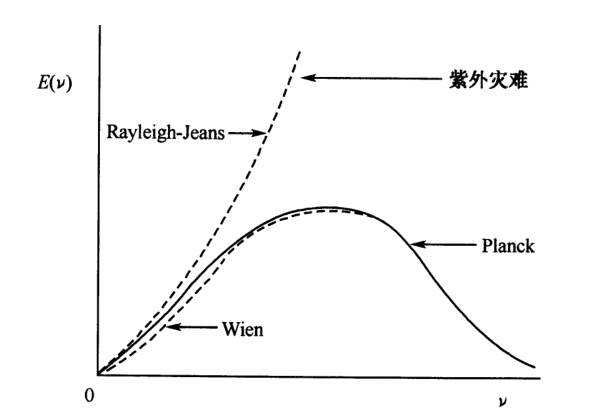
\includegraphics[scale=0.8]{fig/blacknu.jpg}
	\caption{这是一张图}
\end{figure}

\begin{figure}[H]
	\centering
	\begin{subfigure}[b]{0.45\textwidth}
		\centering
		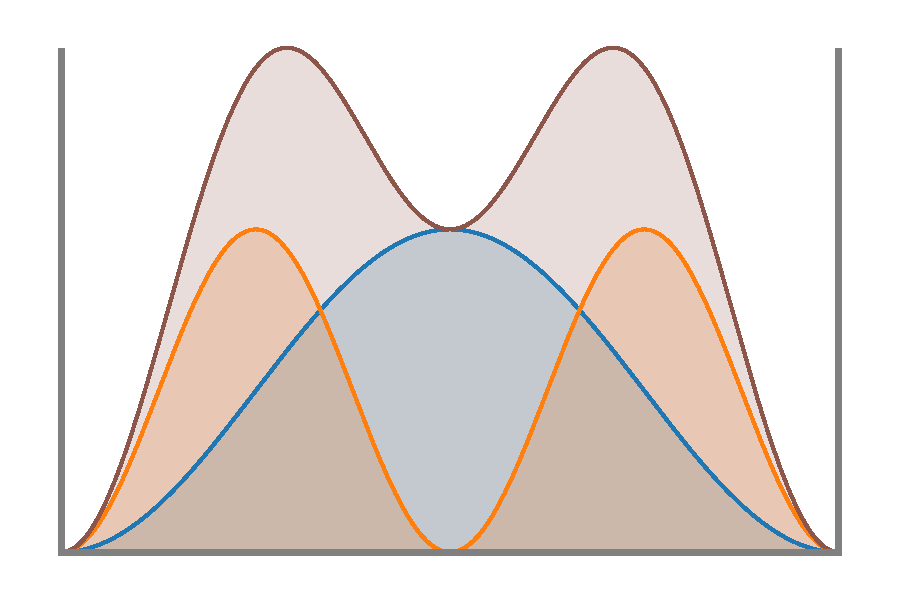
\includegraphics[scale=0.45]{./fig/13-box.pdf}
		\caption{1,3-丁二烯}
	\end{subfigure}
	\begin{subfigure}[b]{0.45\textwidth}
		\centering
		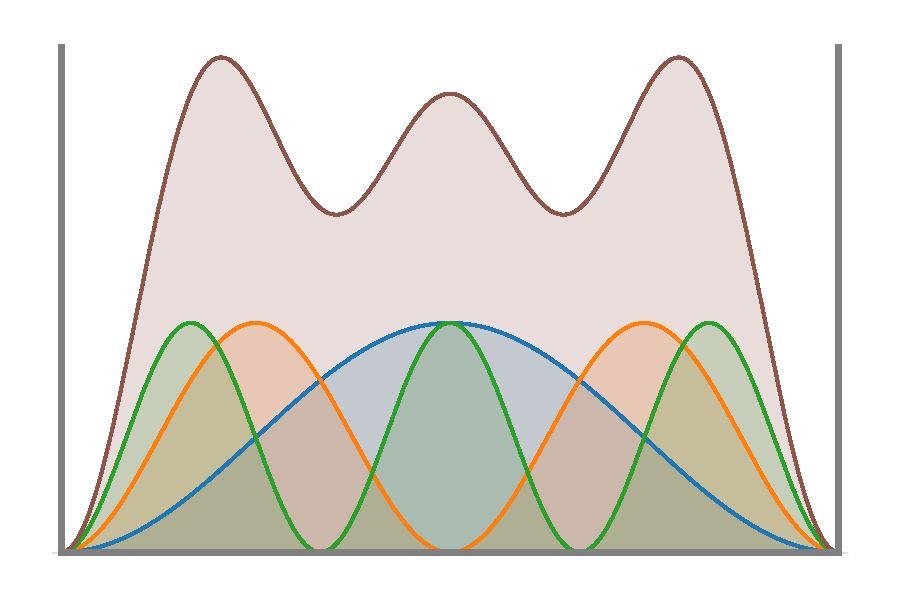
\includegraphics[scale=0.45]{./fig/15-box.pdf}
		\caption{1,3,5-己三烯}
	\end{subfigure}
	\caption{这是两张图}
\end{figure}

\subsection{TikZ图}
\begin{figure}[H]
	\centering
	\begin{tikzpicture}[scale=3,>={Stealth[round]}]
	\draw [fill, AliceBlue] (-1.1, -0.2) -- (-1.1, 0) --++ (1.1, 0) --++ (0, 0.3) --++ (1, 0) --++ (0, -0.3) --++ (1.1, 0) --++ (0, -0.2);
	% Axis
	\draw [->] (-1.1, 0) -- (2.1, 0) node[right] {$x$};
	\draw [->] (0, -0.2) -- (0, 0.8) node[above] {$V(x)$};
	\node at (0, 0) [below left] {$O$};
	% Potential
	\draw [DarkSlateBlue,ultra thick,join=round] (-1, 0) --++ (1, 0) --++ (0, 0.3) --++ (1, 0) --++ (0, -0.3) node[below] {$l$} --++ (1, 0);
	%\draw [Crimson,ultra thick,dotted] (-1.1, 0.2) -- (2.1, 0.2);
	% Wave
	\draw [->,Chocolate,decorate,decoration=snake] (-0.4, 0.7) node[left] {$A_1 e^{i k_1 x}$} --++ (0.3, 0);
	\draw [->,DarkCyan,decorate,decoration=snake] (-0.1, 0.5) --++ (-0.3, 0) node[left] {$B_1 e^{- i k_1 x}$};
	%\draw [->,Chocolate,decorate, rounded corners] (0.6, 0.7)  node[left] {$C_2 e^{\kappa_2 x}$}  arc[start angle=0, delta angle=90] -- ++(0.3, 0.2);
	\draw [->,Chocolate,decorate] (0.6, 0.7)  node[left] {$C_2 e^{\kappa_2 x}$}  parabola ++(0.3, 0.15);
	\draw [->,DarkCyan,decorate] (0.6, 0.5) node[left] {$D_2 e^{- \kappa_2 x}$} parabola ++ (0.3, -0.15) ;
	\draw [->,Chocolate,decorate,decoration=snake] (1.6, 0.7) node[left] {$A_3 e^{i k_1 x}$} --++ (0.3, 0);
	\draw [->,DarkCyan,decorate,decoration=snake,densely dotted] (1.9, 0.5) --++ (-0.3, 0) node[left] {$B_3 e^{- i k_1 x}$};
	\end{tikzpicture}
\end{figure}

\section{杂项}
脚注
\begin{note}	
	但是在量子力学中并不排除会使用某些不能归一化的波函数。\footnote{这是一个脚注}
\end{note}




引用公式,\eqref{braket}。需要多编译一次。

\subsection{一些自定义命令}

\end{document}
